\chapter{Self-interacting dark matter}
\label{sec:sidm}

\section{Motivations}
We have previously discussed the small-scale problems observed with the
$\Lambda$CDM paradigm. One of the richest potential solutions comes when
considering self-interacting dark matter (SIDM) models. These models introduce
new mechanisms by which dark matter particles can interact with each other,
beyond the gravitational interaction allowed by the CDM model.

SIDM models were first proposed in 1999 by Spergel and Steinhardt, who compiled
obesrvational evidence for its existence~\cite{spergel_observational_2000}.
They also performed initial simulations which found that SIDM models tend to
give rise to cored halso and different small-scale structures, indicating a
potential solution to the core-cusp and other small-scale
problems~\cite{dave_halo_2001}. This sparked a number of other studies of
SIDM simulations which used various observational data to place constraints
on the self-interaction cross section of the dark matter particles. These
studies greatly constrained the cross section-to-mass ratio to a degree where
the impact of self-interaction would be too small to solve the small-scale
problems. As such, SIDM models fell out of favor for a while.

More recently, however, higher resolution simulations have produced revisions to
the original constraints that are significantly looser, improving the viability
of SIDM and re-igniting the study of these models~\cite{tulin_dark_2018}.
Comparisons to observations of dwarf galaxies have shown that a self-interaction
cross section-to-mass ratio of $\sigma / m \sim 0.5$-1 cm$^2$/g is needed.
Studies of massive clusters, however, showed that something closer to $\sigma /
m \sim 0.1$ cm$^2$/g is needed. Together, these imply that the self-interaction
cross section must be velocity-dependent, such that it can admit the proper
cross sections on both scales, ruling out simple SIDM models such as a
self-coupled scalar.

The only property of these self-interacting dark matter models that will come to
strongly affect astrophysical observation is the cross section-to-mass ratio
$\sigma/m$ for two-to-two self-scattering. On astrophysical scales, the
scattering rate per particle $\Gamma$ scales as $\Gamma \sim (\sigma/m)
\rho(r) v_{\text{rms}}$, where $\rho$ is the local mass density and
$v_\text{rms}$ is the r.m.s.~speed of DM particles~\cite{robles_sidm_2017}.
As such, we can consider SIDM models in a general way when performing N-body
simulations. This also yields a large freedom in the models which can be
consistent with observation. Two of the most prominent models are discussed
below. 

\section{Particle physics models}
With little known about the precise nature of dark matter, there is a seemingly
infinite number of possible theories to explore. We will discuss two of the
most prominent kinds of theories.

\subsection{Light mediator}
The first is a rather simple theory that admits a rich potential phenomeonology.
We let the dark matter particle be $\chi$, a fermion with mass $m_\chi$, charged
under a spontaneously broken $U(1)$ symmetry~\cite{tulin_dark_2018}. Let the
resulting gauge boson be $\phi$ with mass $m_\phi$. Depending on the specific
theory, $\phi$ may be a scalar or vector particle. The interaction term of the
Lagrangian would then be a Yukawa coupling
\begin{equation}
    \mathcal{L}_\text{int} = \left\{ \begin{array}{cl}
        g_\chi \chibar \gamma^\mu \chi \phi_\mu & (\text{vector mediator}) \\
        g_\chi \chibar \chi \phi & (\text{scalar mediator,})
    \end{array} \right.
\end{equation}
where we let the coupling constant be $g_\chi$. In the non-relativistic limit,
such an interaction is described by the Yukawa 
potential~\cite{tulin_beyond_2013, tulin_resonant_2013}
\begin{equation}
    V(r) = \pm \frac{\alpha_\chi}{r} e^{-m_\phi r},
\end{equation}
where $\alpha_\chi \equiv g_\chi^2 / 4\pi$ is the dark fine structure constant,
and the $\pm$ is set depending on whether the potential is attractive or
repulsive.\footnote{For a scalar $\phi$, the potential is always attractive and
the sign is $(-)$. For a vector $\phi$, the potential is attractive $(-)$ for
$\chi\chibar$ scattering and repulsive $(+)$ for $\chi\chi$ and $\chibar\chibar$
scattering.}

We can use the non-relativistic Yukawa potential above to obtain the Born
differential cross section in the limit that $\alpha_\chi m_\chi / m_\phi \ll
1$. The final result is~\cite{tulin_dark_2018}
\begin{equation}
    \frac{d\sigma}{d\Omega}
    = \frac{\alpha_\chi^2 m_\chi^2}{\left[ m_\chi^2 v_{\text{rel}}^2 (1 - \cos\theta) / 2 + m_\phi^2 \right]^2}.
\end{equation}
An important implication of this result is that we must have $m_\phi > 0$. If
instead $m_\phi = 0$, we would see $d\sigma/d\Omega \propto
v_{\text{rel}}^{-4}$. This velocity dependence is far too strong at small
velocities to admit a solution consistent with observation. A small but nonzero
$m_\phi$, however, allows us to ``soften'' this velocity-dependence, admitting a
more consistent model.

The differential cross section may also be analytically computed in the
classical limit, $m_\chi v_{\text{rel}} / m_\phi \ll 1$. However, exploring this
model over a wider range of parameter space requires us to leave the regimes
where the Born and classical approximations hold. Analytic results which hold
generally outside these regimes do not exit, so there has been some work done to
develop methods for approximately obtaining the results. One such method uses an
the Hulthén potential, an approximation of the Yukawa potential. Another uses
non-relativistic partial wave analysis to develop numerical methods that are
accurate across more of phase space. There are other methods that can be
considered as well; a more complete map of these methods can be found
in~\cite{tulin_beyond_2013}.

One can use the approximation methods described above to explore various regions
of phase space and to consider the velocity-dependence of the cross section that
will results. For example, Figure~\ref{fig:sidm} (left) shows the
velocity-dependences of the cross section for an attractive potential in the
limits considered previously, using choices for sample parameters. One can
see that the Yukawa potential with a mediator particle can result in a very
rich variety of velocity dependences, depending on our choice of particle
physics parameters. As such, one can use astrophysical observations to
constrain the phase space of these parameters. An example of such constraints
is given in Figure~\ref{fig:sidm} (right).

This model is admittedly rather simple, but it has been shown
in~\cite{tulin_beyond_2013} that it is possible for it simultaneously
accomodate all important observations and to solve the small-scale problems.

\begin{figure}[t!]
    \centering
    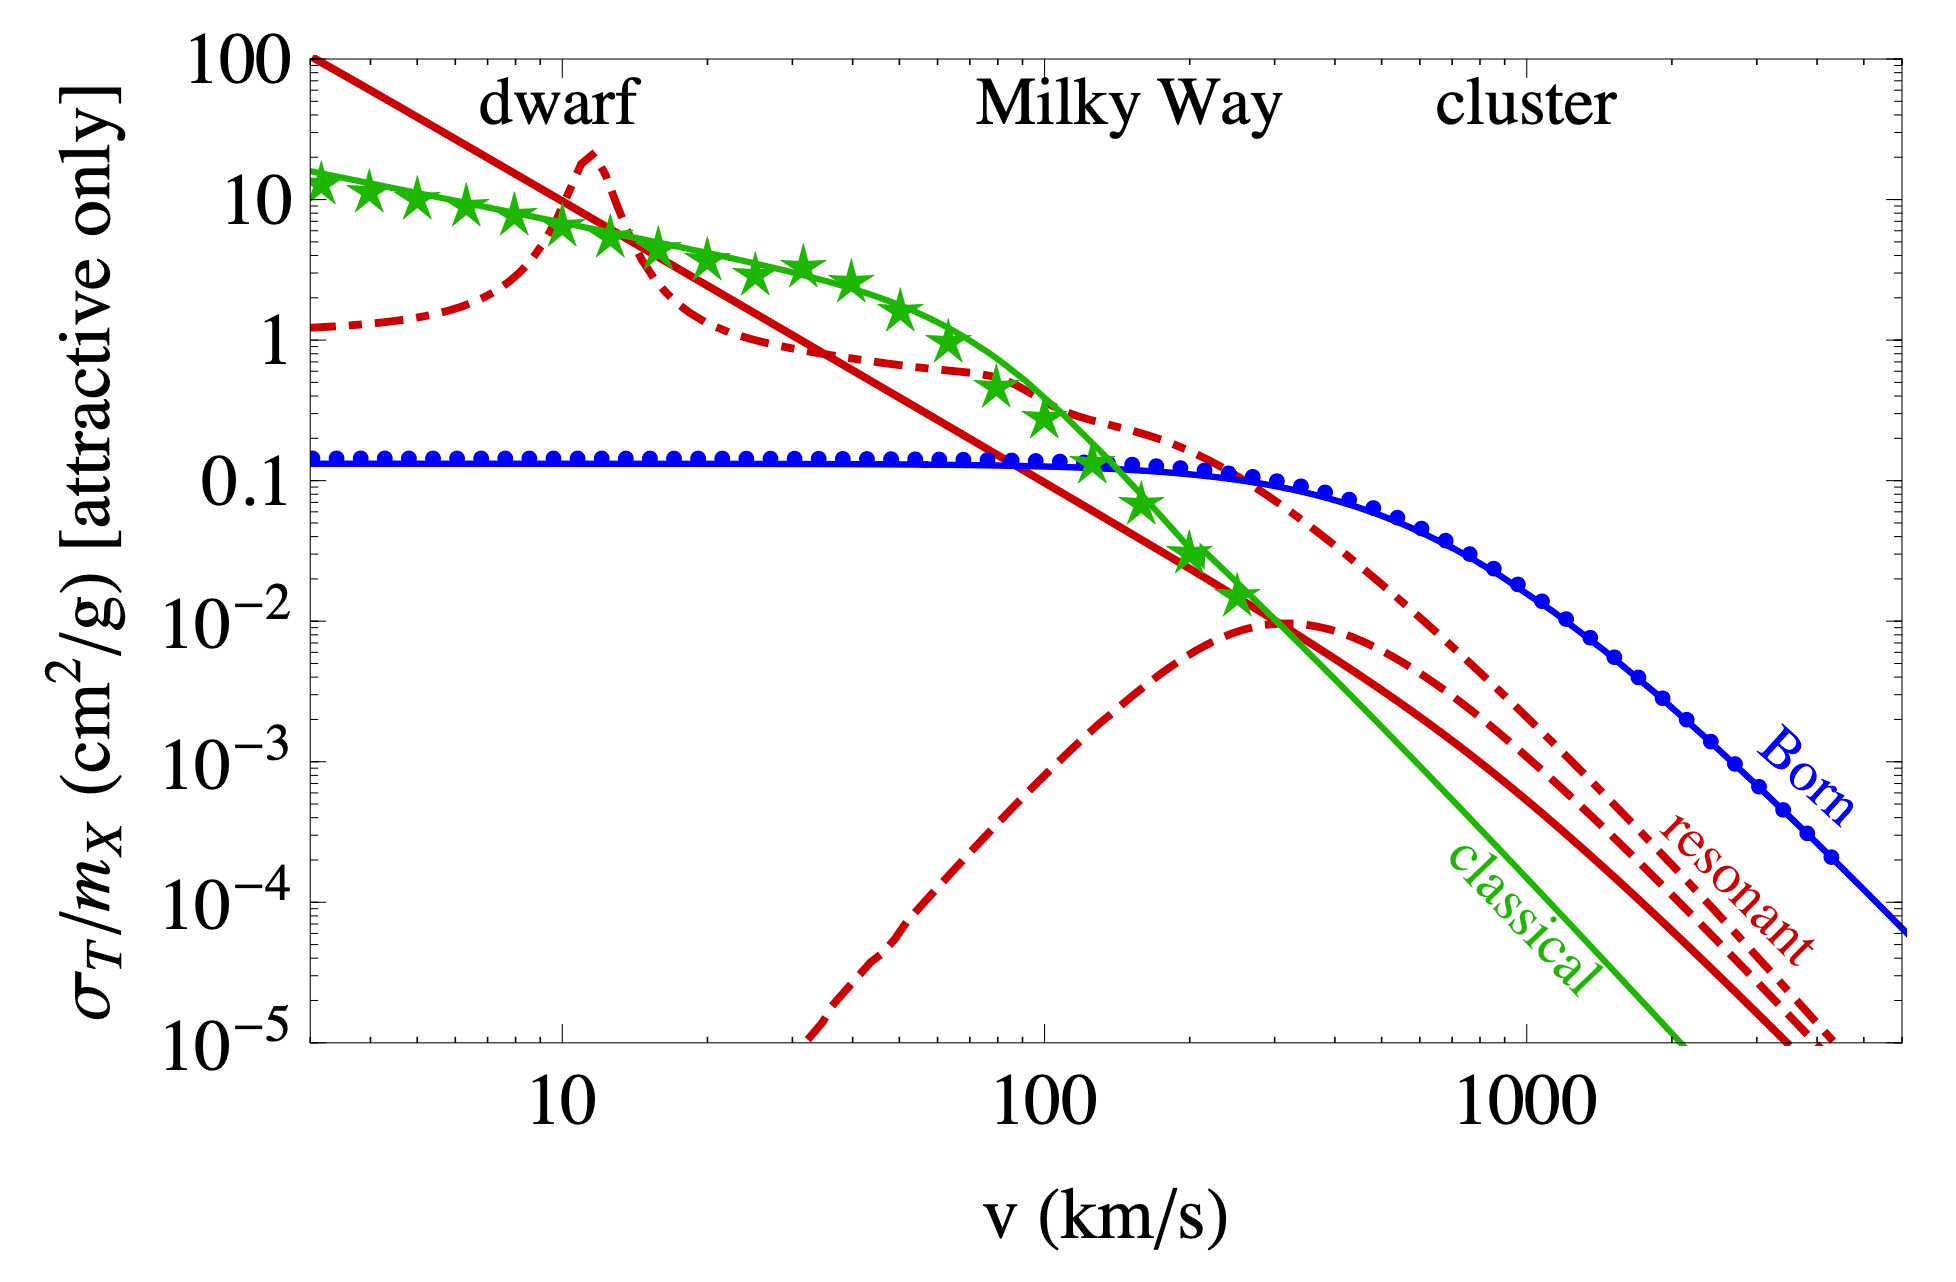
\includegraphics[width=0.45\linewidth]{fig/sigma_vs_vel.png}
    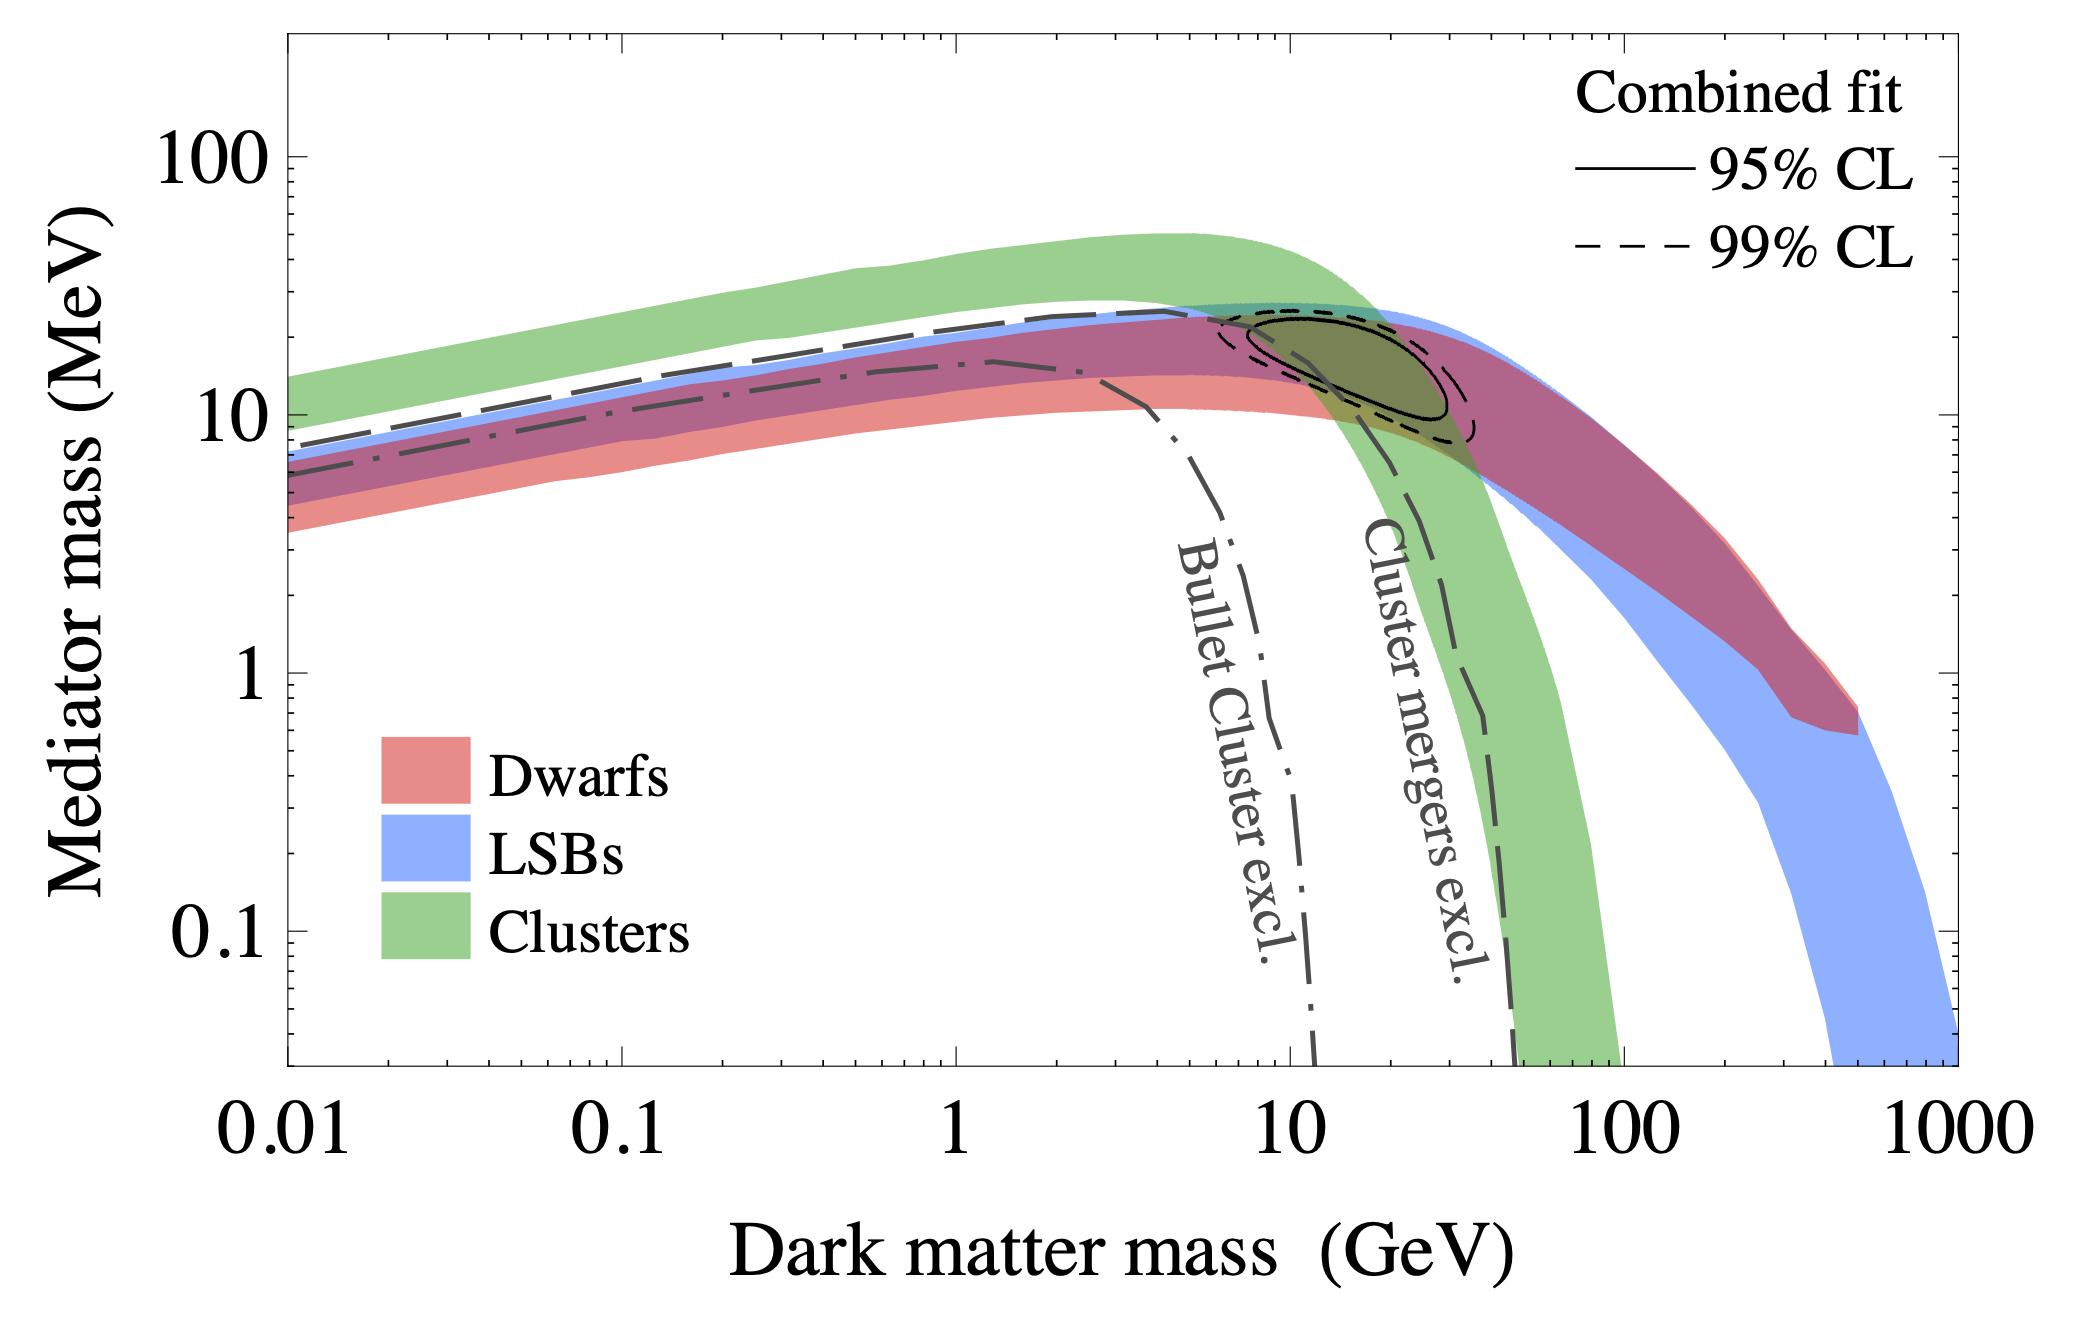
\includegraphics[width=0.45\linewidth]{fig/yukawa_constraint.png}
    \caption{
        (Left) The velocity dependence of $\sigma/m$ for sample parameter values
        ($\alpha_\chi$, $m_\chi$, $m_\phi$) assuming an attractive Yukawa
        potential. The blue, red, and green lines show the differential cross
        section computed under different limits; blue is the Born limit,
        green is classical, and red is the resonant régime, which is
        undiscussed in this paper. Reprinted from~\cite{tulin_resonant_2013}.
        (Right) The parameter space for a repulsive Yukawa potential,
        assuming $\alpha_\chi \approx 1/137$. In colored regions are the
        regions of parameter space preferred by observations from dwarf
        galaxies (red), low surface brightness (LSB) galaxies (blue), and
        galaxy clusters (green). Reprinted from~\cite{kaplinghat_dark_2016}.
    }
    \label{fig:sidm}
\end{figure}


\subsection{Strong interactions}
Some of the richest theories for self-interacting dark matter candidates that
one can consider are non-Abelian gauge theories where the dark matter candidates
arise as composite bound states. In these theories, the self-interaction
manifests as a strong interaction.

The motivation for a considering such a model comes from our experience with QCD
and the visible sector~\cite{kribs_review_2016}. For a dark matter model to be a
good candidate, it must be stable over the lifetime of the Universe and be
neutral under standard model phenomena. Further, we desire models in which the
models exhibit strong self-interactions. These are all properties exhibited by
particles in the visible sector under QCD, so it makes sense to consider a
similar theory to describe our dark matter candidate. However, we do not
necessarily know the gauge group or particle properties of dark matter, leaving
us a great freedom to vary the model significantly. Many of the resulting models
thus have interesting and unique new physics, though these details are greatly
model-dependent.

The primary free parameters of models of this kind are the confinement scale,
$\Lambda$, and the dark quark mass(es). In the event that our ``dark QCD''
contains no analogue to electromagentic/weak interactions, meson-like bound
states of the dark quarks could be stable~\cite{cline_composite_2014}. These
mesons can be classified as loosely pion-like, where $m \ll \Lambda$, or
quarkonium-like, where $m \gg \Lambda$~\cite{kribs_review_2016}. There are
several proposed models for each of these scenarios; one of the more well-known
is the strongly-interacting massive particle, or SIMP, where the dark matter
candidate is pion-like and many non-Abelian theories are possible.

Our non-Abelian model may instead look quite similar to visible QCD, wherein the
primary stable bound states are baryonic in nature. In~\cite{kribs_review_2016},
it is noted that the advantage of such models is that ``dark matter is
automatically sufficiently stable, and no further ultraviolet model-building is
needed.'' One such dark baryon model is ``Stealth Dark Matter,'' proposed by the
LSD collaboration, which is a scalar dark baryon under a confining $SU(4)$
theory. This theory is named \textit{stealth} dark matter because it is found
that the baryons are safe from direct detection, though it does predict a
spectrum of lighter meson particles that would be possible to detect at
colliders~\cite{kribs_review_2016}.

The third class of candidate particles that has received attention are dark
glueballs. Glueballs are bound states of only gluons, and are predicted to exist
in QCD but are very difficult to detect. Dark glueballs would then be bound
states of dark gluons. Such a model is possible if all the dark fermions in the
theory have masses significantly larger than $\Lambda$. In this case, glueballs
may become stable under an accidental symmetry like baryons, allowing them to be
the primary dark matter candidate.

The observables that could result from the above considerations are as diverse
as the models themselves. One aspect of these models that we have not considered
is what the interactions with the standard model could look like. Some models
predict the dark matter candidate to be neutral under standard model
interactions, but its constituents to be charged. In such a case, the model
would have a coupling to the photon, and it would be possible to directly detect
the particle. We may also consider the case where our theory predicts
fundamental fermions. It is plausible that these fermions would obtain at least
part of their mass through a coupling to the Higgs boson, again providing a
mechanism by which we could directly detect the particles. Kribs and Neil
provide more details of these observables, as well as collider-specific results,
in \cite{kribs_review_2016}.


% \section{Astrophysical impacts}
% The most important result from any of the above models is the cross
% section-to-mass ratio, $\sigma/m$ for two-to-two self-scattering. On
% astrophysical scales, the scattering rate per particle $\Gamma$ scales as
% $\Gamma \sim (\sigma/m) \rho(r) v_{\text{rms}}$, where $\rho$ is the local
% mass density and $v_\text{rms}$ is the r.m.s.~speed of DM
% particles~\cite{robles_sidm_2017}.
% 
% \todo{Talk about some of Robles et al.'s results.}
